\documentclass[a4paper]{article}

%% Language and font encodings
\usepackage[english]{babel}
\usepackage[utf8x]{inputenc}
\usepackage[T1]{fontenc}
%\usepackage{ebgaramond}
%\usepackage{kpfonts}
%% Sets page size and margins
\usepackage[a4paper]{geometry}

%% Useful packages
\usepackage{ascmac}
\newdimen\tbaselineshift
\usepackage{amsmath}
\usepackage{graphicx}
\usepackage{xspace}
\usepackage{color}
\usepackage[titletoc,title]{appendix}

\usepackage[colorinlistoftodos]{todonotes}
\usepackage[colorlinks=true, allcolors=blue]{hyperref}
\addto{\captionsenglish}{\renewcommand{\abstractname}{Preface}}
%\newcommand{\lam}{\mbox{\Lambda (1405)}\xspace}

\newcommand{\pS}{\mbox{$\pi^{\pm}\Sigma^{\mp}$}\xspace}
\newcommand{\reaction}{\mbox{$\Lambda(1405)\rightarrow \pi^{\pm}\Sigma^{\mp}$}\xspace}
\newcommand{\mev}{\mbox{MeV}\xspace}
\newcommand{\mevc}{\mbox{MeV/$c~$}\xspace}
\newcommand{\mevee}{\mbox{MeVee}\xspace}
\newcommand{\gev}{\mbox{GeV}\xspace}
\newcommand{\gevc}{\mbox{GeV/$c~$}\xspace}
\newcommand{\gevcsq}{\mbox{GeV/$c^{2}~$}\xspace}
\newcommand{\sqs}{\mbox{$\sqrt{s}$}\xspace}

\hypersetup{
  colorlinks=true,       % false:boxed links;true:colored links
    linkcolor=blue,          % color of internal links (change box color with linkbordercolor)
    citecolor=green,        % color of links to bibliography
    filecolor=magenta,      % color of file links
    urlcolor=cyan           % color of external links
}


\graphicspath{
  %
  {./},%
  {./fig/}%
}



%\newcommand{\updateinfo}[1][\today]{\par\vfill\hfill{\scriptsize\color{gray}Last updated on #1}}
\newcommand{\updateinfo}[1][\today]{{\par{\color{gray}Last updated on #1}}}
\pagenumbering{roman}

\title{Momentum transfer dependence of the cross section of the $\Lambda(1405)$ in E31-2nd }
\author{Hidemitsu Asano}
\date{}

\makeindex

\begin{document}
\maketitle
\vspace{4em}
\begin{abstract}
\noindent This note details the analysis of the $\Lambda(1405)\rightarrow \pS $ invariant mass spectra produced in the $d(K^-,\Lambda(1405))n$ reaction in E31-2nd. The main goal of this analysis is to measure the cross section of the $\Lambda(1405)$ vs the momentum transfer of the reaction.
\end{abstract}
\tableofcontents

\clearpage
\listoffigures

\clearpage
\listoftables

\clearpage
\pagenumbering{arabic}

\section{Introduction}
The main goal of this analysis is to measure momentum transfer dependence of the cross section of the $\Lambda (1405)$ via the $(K^-,n)$ reaction on deuteron target.
The momentum transfer dependence can be related to the size of the resonance.
This analysis is inspired by J-PARC E15 analysis \cite{Sada:2016nkb,Ajimura:2018iyx}.

In this analysis, invariant mass of the $\Lambda (1405)$ is reconstructed by detecting $\pi^{+},\pi^-$ and the neutron by the CDS, namely:

\begin{eqnarray}
\Lambda (1405) & \rightarrow & \Sigma^+\pi^-  \rightarrow {\pi^-\pi^+}n \quad (16.1\%)  \nonumber \\
               & \rightarrow & \Sigma^-\pi^+  \rightarrow {\pi^+\pi^-}n \quad (33.3\%)
\end{eqnarray}
Number in parenthesis shows a branching ratio.
Here, the forward neutron is identified from the missing mass of 
$d(K^-,\pi^+\pi^-n)$X reaction. In this way, we can widely measure the momentum transfer of the \reaction reaction. 
The momentum transfer ($q$) is defined by, $q=|\overrightarrow{K_{\mbox{beam}}} - \overrightarrow{n_{\mbox{miss}}}|$.

%\begin{equation} \label{pole} 
%  \frac{d^2 \sigma _X}{dM_{inv.\Lambda (1405)}dq_{\Lambda p}} \propto \rho _{3}(\Lambda p n) \times     \frac{(\Gamma _X/2)^2}{(M_{inv.\Lambda p}-M_{X})^2 + (\Gamma _{X} /2)^2 } \times  | \exp{(-q_{    \Lambda p}^2/2Q_{X}^2)}|^2 ,
%\end{equation} 

%\todo[inline,color=green]{need to take into account spin parity? -> perhaps, no. They are just averaged out}
\begin{equation} \label{formfactor} 
 % \frac{d^2 \sigma _X}{dM_{\Sigma \pi} dq_{\Sigma \pi}} \propto \rho _{3}(\Sigma \pi n) \times     \frac{(\Gamma _X/2)^2}{(M_{\Sigma \pi}-M_{X})^2 + (\Gamma _{X} /2)^2 } \times  | \exp{(-q_{    \Sigma \pi}^2/2Q_{X}^2)}|^2 ,
  \frac{d^2 \sigma _X}{dM_{\Sigma \pi} dq} \propto \rho _{3}(\Sigma \pi n) \times \frac{(\Gamma _{\Sigma \pi} /2)^2}{(M - M_{\Sigma \pi})^2 + (\Gamma _{\Sigma \pi} /2)^2 } \times  | \exp{(-q^2/2Q_{X}^2)}|^2 ,
\end{equation} 
where $M_{\Sigma \pi}$ is the invariant mass of $\Sigma \pi$ and $q_{\Sigma \pi}$ is defined as $ q_{\Sigma \pi} \equiv |p_\Sigma| + |p_\pi| $ , which is the momentum transfer of the reaction. $\rho_{3}(\Sigma \pi n) $ is the three body phase space. $\Gamma_X$ is the decay-width of Breit-Wigner peak. $Q_X$ is a free parameter which can be interpreted as the form factor parameter of the pole.  
If the $Q_X \to \infty $, the formula above becomes point-like interaction.

\begin{table}[]
  \centering  
  \renewcommand\arraystretch{2}
  \caption{resonaces expected in the $\pi^\pm\Sigma^\mp$ spectra}
  \begin{tabular}{ccccc} \hline
  resonace & mass & $I(J^p)$ & $\bar{K}N$ scattering & B.R.\\ \hline\hline
  $\Lambda(1405)$  &  ?     & 0($\frac{1}{2}^-)$  & S-wave & 100\% \\ \hline
  $\Sigma(1385)^0$   & $1383.7 \pm 1.0$ MeV & $1(\frac{3}{2}^+)$ & P-wave & 11.7 $\pm$ 1.5\% \\ \hline
  $\Lambda(1520)$  & $1519.5 \pm 1.0$ MeV & $0(\frac{3}{2}^-)$ & D-wave & 42 $\pm$ 1\% \\ \hline
  \end{tabular}
\end{table}


\subsection{Review of $\Lambda (1405)$ physics}





\section{Experimental setup}
\subsection{new Backward Proton chamber (BPC)}
From Run74, the new Backward Proton Chamber (BPC) was installed in the CDS. The new BPC is used as a vertex detector in front of the target and tracking detector for backward protons.


The BPC is a circular planer chamber whose size is 


\subsection{magnet setting}

\subsection{Deuteron target}

\subsection{DAQ}
The number of SMP is 11. 


\subsection{trigger scheme}




\section{Simulation}
The purpose of those MC simulation is as follows:
\begin{itemize}
\item Acceptance Correction
\item Kinematic Fit
\end{itemize}

\begin{table}[]
  \centering
  \caption{simulation setup}
  \begin{tabular}{l|l} \hline
  GEANT4 version & 4.10.01p1   \\ \hline\hline
  Physics list  &  QGSP\_BERT\_HP   \\ \hline\hline
  Beam Momentum & 1.000 GeV/c (fixed)  \\ \hline\hline 
  \end{tabular}
\end{table}
$\Sigma^+\pi^- n$ and $\Sigma^-\pi^+ n$ events are generated with isotropic phase-space distribution.

\begin{figure}
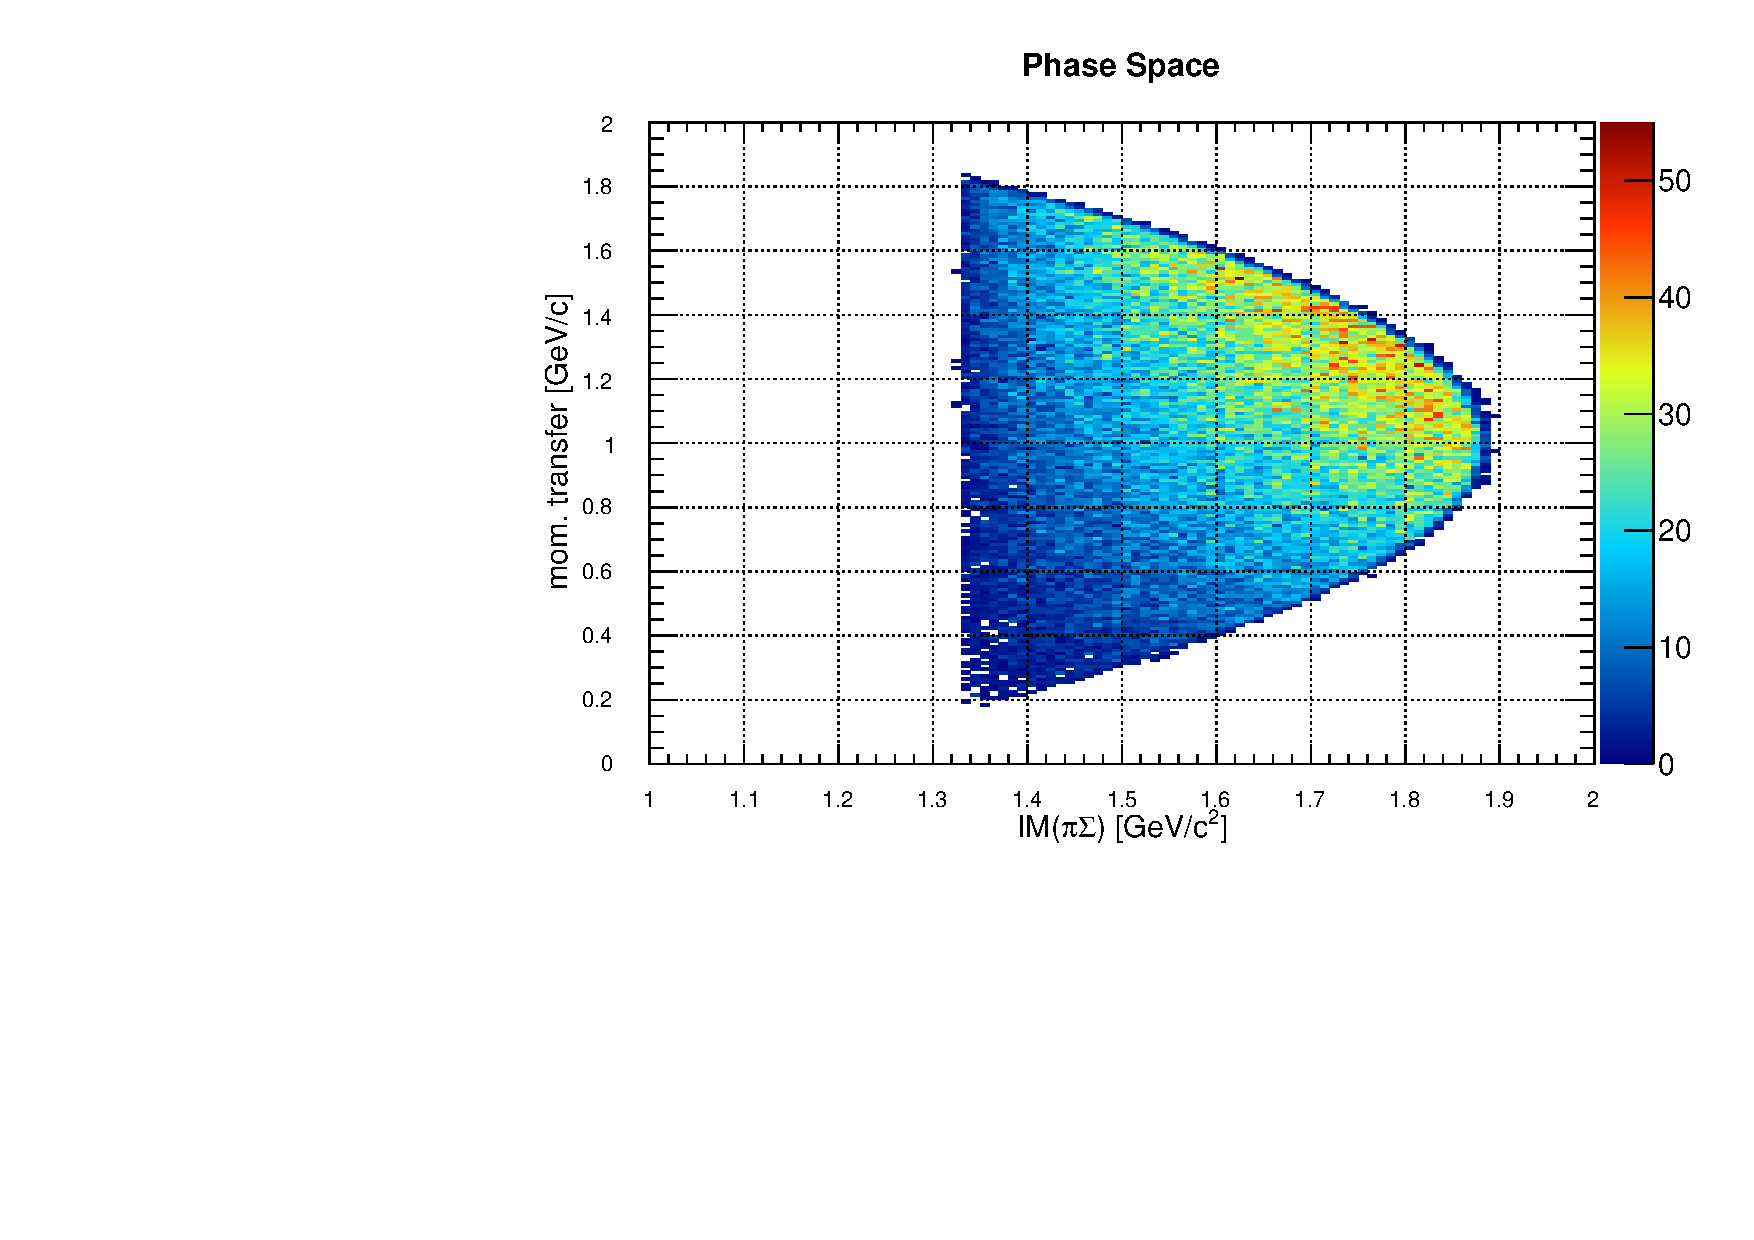
\includegraphics[width=0.45\linewidth]{PSSp.pdf}
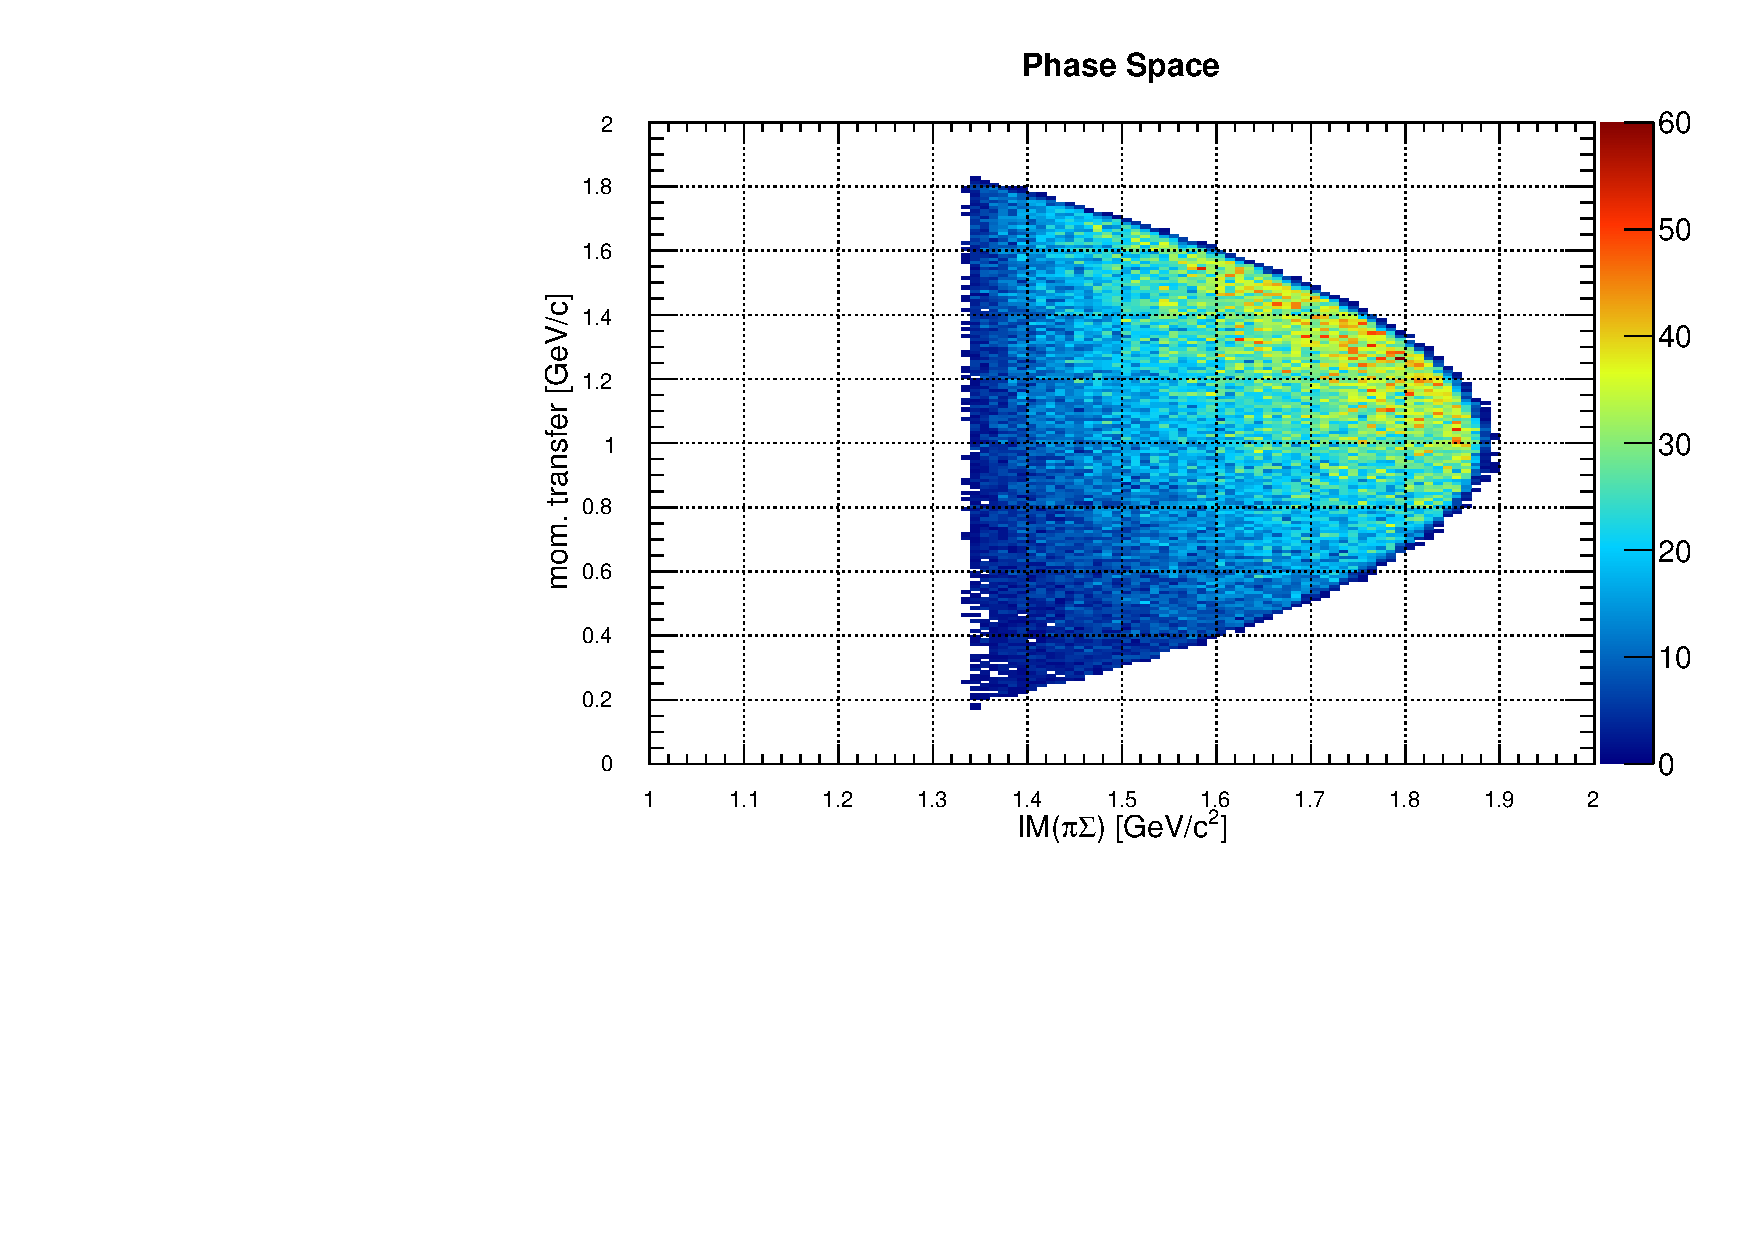
\includegraphics[width=0.45\linewidth]{PSSm.pdf}
\caption{Phase Space distribution of $\Sigma^+$ mode (left) and $\Sigma^-$ mode (right).}
\end{figure}




\subsection{Covarinace matrix of the kinematic fit}




\section{ \reaction invariant mass analysis}
\subsection{overview}


\subsection{Event Selection}
The following event selection by the CDS is made prior to the beam line analysis to reduce CPU time.
\begin{itemize}
\item \# of CDH segments fired == 3
\item \# of good CDC tracks == 2
\item $\pi^+$ and $\pi^-$ are found
\end{itemize}
Here, clustering of CDH hits are not being made.

\subsection{CDH analysis}





\subsection{Beam Analysis}
\subsubsection{Analysis Cuts}

\begin{figure}
\includegraphics[width=\linewidth]{fig/hist2.pdf}
\caption{Hit multiplicity of BHD}
\end{figure}
\begin{figure}
\includegraphics[width=\linewidth]{fig/hist3.pdf}
\caption{Hit multiplicity of T0}
\end{figure}


\begin{figure}
\includegraphics[width=\linewidth]{fig/hist4.pdf}
\caption{Phase Space distribution of $\Sigma^+$ mode (left) and $\Sigma^-$ mode (right).}
\end{figure}

\begin{figure}
\includegraphics[width=\linewidth]{fig/hist5.pdf}
\caption{Phase Space distribution of $\Sigma^+$ mode (left) and $\Sigma^-$ mode (right).}
\end{figure}


\begin{figure}
\includegraphics[width=\linewidth]{fig/hist6.pdf}
\caption{Phase Space distribution of $\Sigma^+$ mode (left) and $\Sigma^-$ mode (right).}
\end{figure}

\begin{figure}
\includegraphics[width=\linewidth]{fig/hist7.pdf}
\caption{Phase Space distribution of $\Sigma^+$ mode (left) and $\Sigma^-$ mode (right).}
\end{figure}

\begin{figure}
\includegraphics[width=\linewidth]{fig/hist8.pdf}
\caption{Phase Space distribution of $\Sigma^+$ mode (left) and $\Sigma^-$ mode (right).}
\end{figure}

\begin{figure}
\includegraphics[width=\linewidth]{fig/hist9.pdf}
\caption{Phase Space distribution of $\Sigma^+$ mode (left) and $\Sigma^-$ mode (right).}
\end{figure}

\begin{figure}
\includegraphics[width=\linewidth]{fig/hist10.pdf}
\caption{Phase Space distribution of $\Sigma^+$ mode (left) and $\Sigma^-$ mode (right).}
\end{figure}

\begin{figure}
\includegraphics[width=\linewidth]{fig/hist11.pdf}
\caption{Phase Space distribution of $\Sigma^+$ mode (left) and $\Sigma^-$ mode (right).}
\end{figure}

\begin{figure}
\includegraphics[width=\linewidth]{fig/hist12.pdf}
\caption{Phase Space distribution of $\Sigma^+$ mode (left) and $\Sigma^-$ mode (right).}
\end{figure}

\begin{figure}
\includegraphics[width=\linewidth]{fig/hist13.pdf}
\caption{Phase Space distribution of $\Sigma^+$ mode (left) and $\Sigma^-$ mode (right).}
\end{figure}

\begin{figure}
\includegraphics[width=\linewidth]{fig/hist14.pdf}
\caption{Phase Space distribution of $\Sigma^+$ mode (left) and $\Sigma^-$ mode (right).}
\end{figure}

\begin{figure}
\includegraphics[width=\linewidth]{fig/hist15.pdf}
\caption{Phase Space distribution of $\Sigma^+$ mode (left) and $\Sigma^-$ mode (right).}
\end{figure}

\begin{figure}
\includegraphics[width=\linewidth]{fig/hist16.pdf}
\caption{Phase Space distribution of $\Sigma^+$ mode (left) and $\Sigma^-$ mode (right).}
\end{figure}

\begin{figure}
\includegraphics[width=\linewidth]{fig/hist17.pdf}
\caption{Phase Space distribution of $\Sigma^+$ mode (left) and $\Sigma^-$ mode (right).}
\end{figure}

\begin{figure}
\includegraphics[width=\linewidth]{fig/hist18.pdf}
\caption{Phase Space distribution of $\Sigma^+$ mode (left) and $\Sigma^-$ mode (right).}
\end{figure}

\begin{figure}
\includegraphics[width=\linewidth]{fig/hist19.pdf}
\caption{Phase Space distribution of $\Sigma^+$ mode (left) and $\Sigma^-$ mode (right).}
\end{figure}

\begin{figure}
\includegraphics[width=\linewidth]{fig/hist20.pdf}
\caption{Phase Space distribution of $\Sigma^+$ mode (left) and $\Sigma^-$ mode (right).}
\end{figure}

\begin{figure}
\includegraphics[width=\linewidth]{fig/hist21.pdf}
\caption{Phase Space distribution of $\Sigma^+$ mode (left) and $\Sigma^-$ mode (right).}
\end{figure}



\subsubsection{$K^-$ Beam Luminosity}



\subsection{$\pi^{+}$ and $\pi^{-}$ identification by the CDS}


\subsubsection{Target fiducial volume}

\subsubsection{Vertex determination}


\subsection{Data quality assurance}


\subsection{Neutral particle identification by the CDS}
%\todo[inline]{under construction, need to understand Sakuma's method }
\begin{itemize}
\item one CDH segment is fired
\item [charge veto] no CDC hits on layer 14 and on 15 in the angle of $\pm 15^\circ$ from the center of the CDH segment above
\item [isolation cuts] no hits on neighboring CDH segments
\end{itemize}

\subsection{Missing mass analysis in $d(K^-,\pi^+\pi^-n)"X"$ reaction}

\subsection{$K^0$ subtraction}


\subsection{$\Sigma^{\pm}$ identification}
%kinematic fit 

\subsection{Resolution of the IM($n\pi^{+}\pi^{-}$)}

\subsection{Resolution of the momentum transfer of the reaction}

\subsection{Acceptance and Efficiency}
The total acceptance as a function of momentum transfer of the reaction (q) and invariant mass of ($n\pi^+\pi^-$) (IM), $\epsilon_{acc}(\mbox{q,IM})$ is evaluated by GEANT4 simulation.
The $n\Sigma^{\pm}\pi^{\mp}$ 3-body simulated data is generated on deuteron target with the incident beam of 1 GeV/c.
The simulated data is generated almost uniformly in (q,IM) space as shown in fig.\ref{fig:genSpSm}. 
Because by using phase space distribution, I can not get enough statistic in low mass region, I generated probability distribution from phase space simulation and put a filter in the event generator. 
Fig.\ref{fig:probSpSm} shows the probability distribution applied for GEANT4 event generator.

\begin{figure}
\includegraphics[width=0.45\linewidth]{simaccSp1.pdf}
\includegraphics[width=0.45\linewidth]{simaccSm1.pdf}\label{fig:genSpSm}
\caption{generated events distribution of $\Sigma^+$ mode (left) and $\Sigma^-$ mode (right).}
\end{figure}

\begin{figure}
\includegraphics[width=0.45\linewidth]{probSp.pdf}
\includegraphics[width=0.45\linewidth]{probSm.pdf}\label{fig:probSpSm}
\caption{probability distribution used for the GEANT4 event generator.}
\end{figure}



The total acceptance is evaluated as follows,
\[
\epsilon_{\mbox{acc}}(\mbox{q,IM}) = \frac{\mbox{Number of accepted events}}{\mbox{Number of generated events in each (q,IM) bin }}
\]
There are no cuts according to binning of (q,IM) to avoid resolution effect of reconstruction.

The $\epsilon_{\mbox{acc}}(\mbox{q,IM})$ includes the branching ratio of $\Sigma^{\pm}$. 



\subsection{$\Sigma(1385)^{-}$ analysis}
$\Sigma^0 \rightarrow \Sigma^\pm\pi^\mp$ contribution (B.R. $=11.7 \pm 1.5 \%$) to the spectra is estimated by $\Lambda \pi$ decay mode (B.R. $=87.0 \pm 1.5 \%)$.
Because we can not measure $\Sigma^0 \rightarrow \Lambda \pi^0$ decay mode, we measure the following reaction instead,
\begin{eqnarray}
 K^-d \rightarrow \Sigma(1385)^-p \rightarrow \Lambda \pi^- p \rightarrow p\pi^-\pi^-p.
\end{eqnarray}
\subsubsection{Event selection for $K^-d \rightarrow \Sigma(1385)^-p$ analysis}
\begin{itemize}
\item \# of CDH segments fired == 3
\item \# of good CDS track == 3
\item $\pi^+,\pi^-$ and $p$ are found.
\end{itemize}

\subsubsection{$\Lambda$ selection}

\subsubsection{missing mass spectra of $d(K^-,p\pi^-\pi^-$)"X"}

\subsubsection{Acceptance and efficiency of $K^-d \rightarrow \Sigma(1385)^-p$}


\subsection{Systematic Error}









\section{Discussion}



\begin{appendices}
\section{Good Run List}


\end{appendices}


\bibliographystyle{unsrt}
\bibliography{main.bib}

\end{document}
